\documentclass{article}
\usepackage{arxiv}
\usepackage[utf8]{inputenc} % allow utf-8 input
\usepackage[T1]{fontenc}    % use 8-bit T1 fonts
\usepackage{hyperref}       % hyperlinks
\usepackage{url}            % simple URL typesetting
\usepackage{booktabs}       % professional-quality tables
\usepackage{amsfonts}       % blackboard math symbols
\usepackage{amsmath}
\usepackage{graphicx}
\usepackage{nicefrac}       % compact symbols for 1/2, etc.
\usepackage{microtype}      % microtypography
\usepackage{lipsum}

% For usage of LaTeX, see the template: https://www.overleaf.com/latex/templates/style-and-template-for-preprints-arxiv-bio-arxiv/fxsnsrzpnvwc

\title{Understanding Alpha Decay}
\author{
  Yuan-Ru Lin
   \And
  Xing-Yao Qiu
   \And
  Heng Xu
}

\begin{document}
\maketitle

\begin{abstract}
Abstract. change to see if Overleaf-GitHub integration is good, guess it would work
\end{abstract}

\section{Introduction}
We read an article which discuss various method for solving $\alpha$-decay. \cite{understandingAlphaDecay}

\section{Breit-Wigner distribution}
From the experiential exponential decaying law, the square of wavefunction decays exponentially along with time:

$$|\psi(t)|^2 = |\psi(0)|^2 e^{-\Gamma t},$$

where $\Gamma$ is a real number.
Then, for an eigenstate in energy $E_R$, there is a decaying term besides the temporal term $e^{-iE_Rt}$, i.e.,

$$\psi(t) = \psi(0) \ e^{-iE_Rt} \ e^{-\frac{\Gamma}{2} t}.$$ 

In order to see energy dependence, we perform Fourier Transform on the wavefunction:

\begin{align*}
\tilde{\psi}(E)
&= \int \psi(t) e^{iEt} dt \\
&= \int \psi(0) \ e^{-iE_Rt} e^{-\frac{\Gamma}{2} t} e^{iEt} dt\\
&\propto \int e^{[i(E-E_R)-\Gamma/2]t} dt \\
&\propto \frac{1}{(E-E_R)+i\Gamma/2}
\end{align*}

The probability of finding the particle at energy $E$ is then:

\begin{align*}
f(E) &= |\psi(t)|^2 \\
&\propto \frac{1}{(E-E_R)^2+(\Gamma/2)^2}
\end{align*}

Such distribution is called a Breit-Wigner distribution.

\begin{figure}
    \centering
    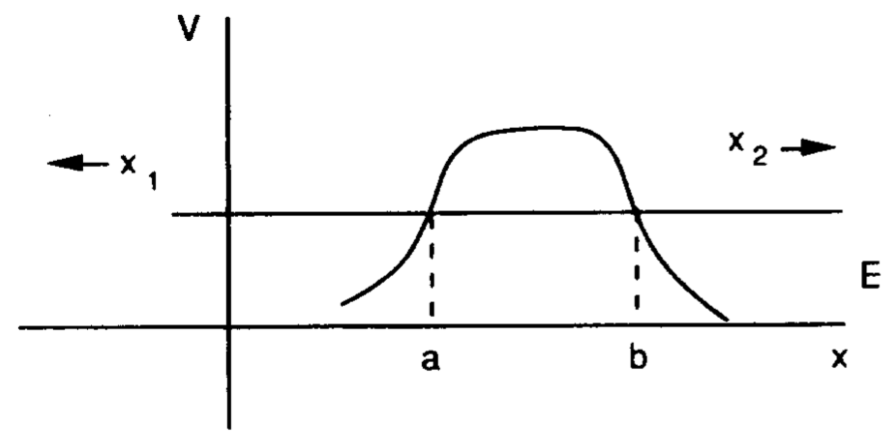
\includegraphics{figures/genericPotential.png}
    \caption{Generic 1-dimensional potential}
    \label{fig:genericPotential}
\end{figure}

\bibliographystyle{unsrt}  
\begin{thebibliography}{1}
\bibitem{understandingAlphaDecay}
George Kour and Raid Saabne.
\newblock Real-time segmentation of on-line handwritten arabic script.
\newblock In {\em Frontiers in Handwriting Recognition (ICFHR), 2014 14th
  International Conference on}, pages 417--422. IEEE, 2014.

\end{thebibliography}


\end{document}
